%Neuer versuch, ein geeignetes Beispiel zu finden
\subsection{Einfaches Beispiel}
\paragraph{Neuer start (der Weg zu einem leichten Beispiel):}
Beginne mit
\[ t^4(t+1)\partial_t^4 + t\partial_t^2+\frac{1}{t}\partial_t+1 \]
\begin{center} 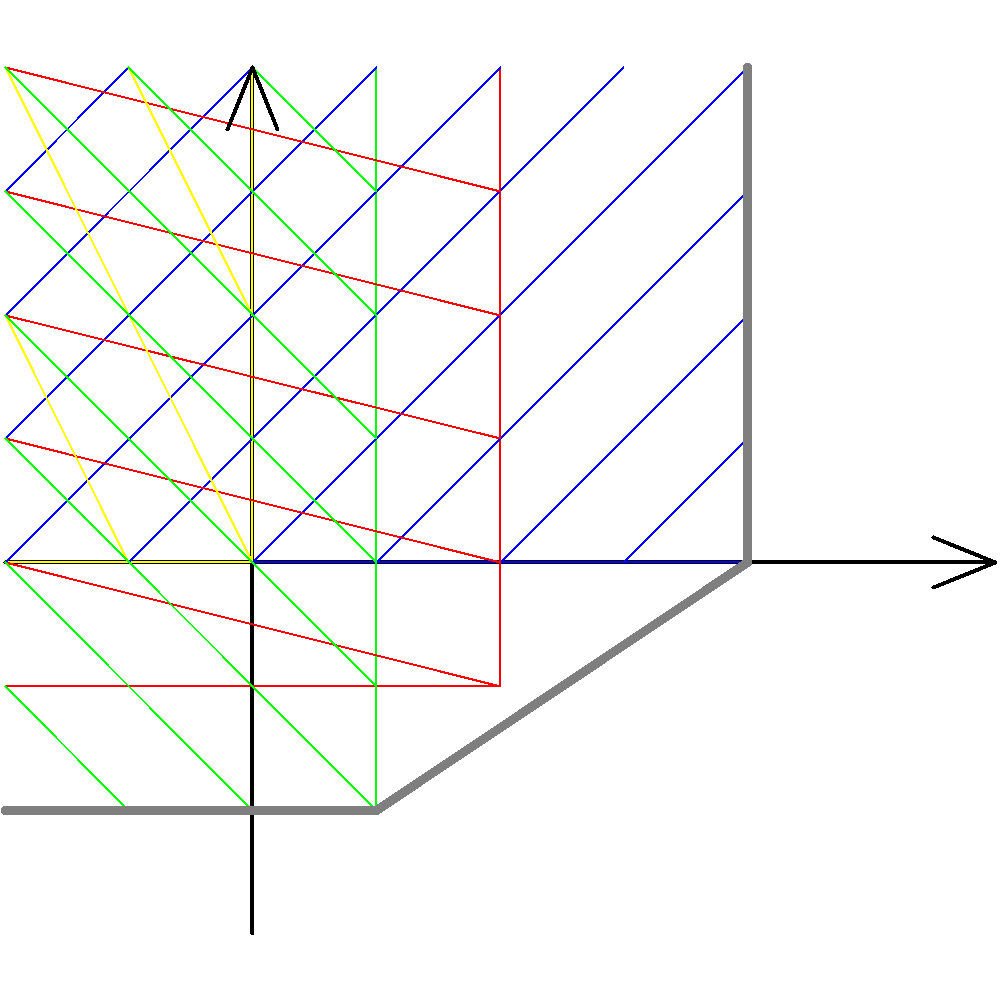
\includegraphics[width=3cm]{beispiele/img/e.png} \end{center}
(von ZulaBarbara Seite 47)
und ignoriere zuerst die Terme, die zum Newton Polygon keinen Beitrag Leisten
\[ t^4\partial_t^4 +\frac{1}{t}\partial_t \]
\begin{center} 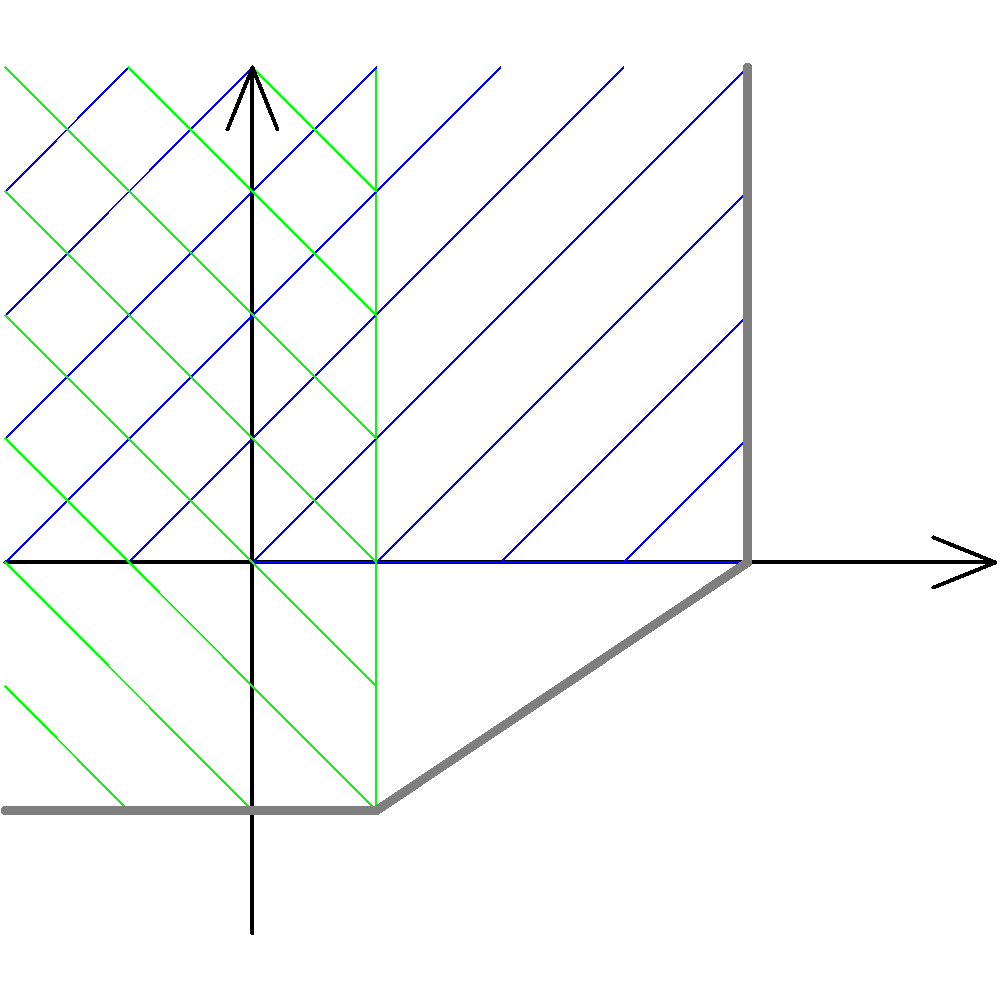
\includegraphics[width=3cm]{beispiele/img/bar_e.png} \end{center}
multipliziere dieses mit $t$ und ändere aber dadurch den assoziierten
Meromorphen Zusammenhang nicht \cite[Chapter 5.1]{sabbah_cimpa90}
\[ P:=t^5\partial_t^4 +\partial_t \]
\begin{center} 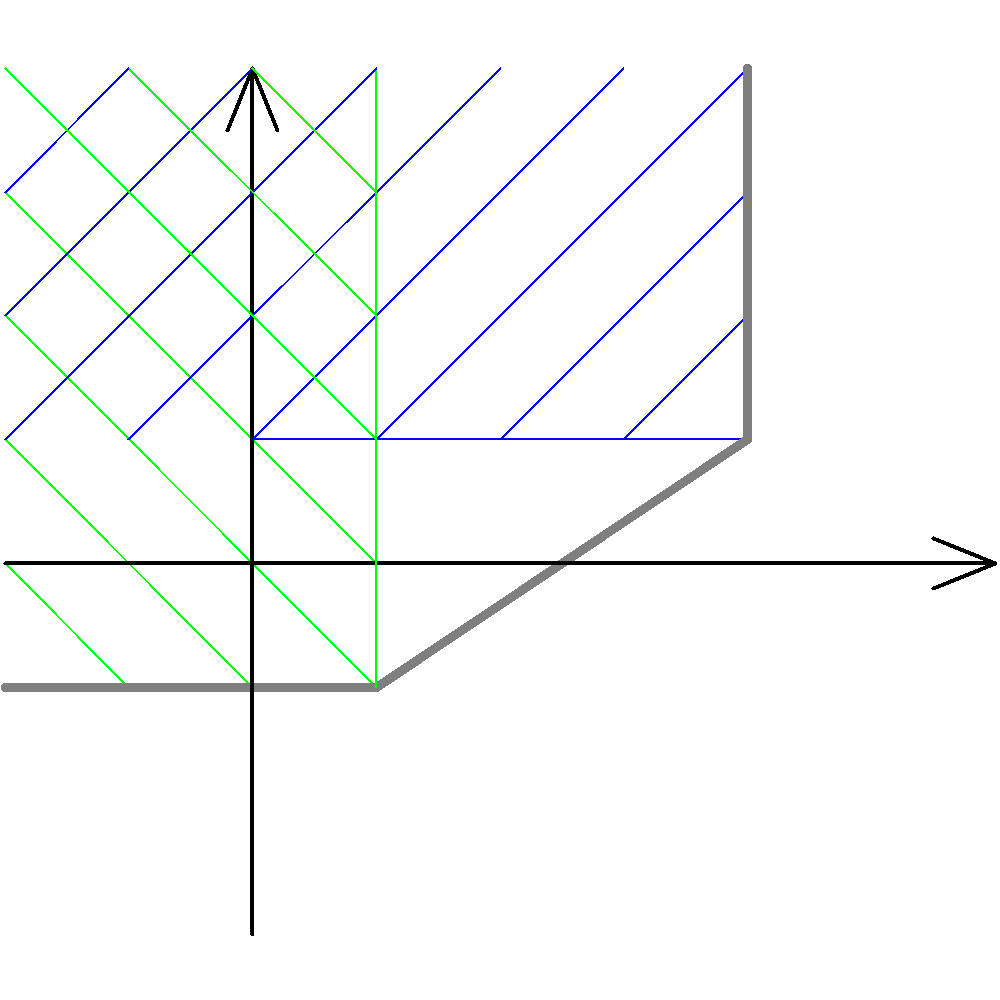
\includegraphics[width=3cm]{beispiele/img/bar_e_times_x.png} \end{center}
und es gilt $\slopes(P)=\{0,\frac{2}{3}\}$. Eliminiere als nächstes nun die
Brüche in den Slopes mittels einem geeignetem Pullback. Da hier der Hauptnenner
$3$ ist bietet sich $\rho:t\mapsto u^3$ für den Pullback an.
\begin{comment}
  Dieser Pullback Multipliziert (indirekt) die Slopes mit $3$,
  \textbf{Quelle?}\\ aber wie wendet man ihn (explizit) an?
\end{comment}

\[ \rho^+P=??? \]
welches die Slopes $\slopes(\rho^+P)=\{0,2\}\subset\Z$ hat. Schreibe nun dieses
$\rho^+P=Q\cdot R$ mit $P,Q\in\Cfu$ wobei gilt $\slopes(Q)=\{0\}$ und
$\slopes(R)=\{2\}$.

Also gilt:
\[
  \hat\cD/(\hat\cD\cdot\rho^+P)\cong
  \hat\cD/(\hat\cD\cdot Q) \oplus  \hat\cD/(\hat\cD\cdot R)
\]

% vim: set ft=tex :
